\section{Behavioral Evaluation}
\label{sec:behavior}
\subsection{Protocol}
Every condition generates the same 12 seeds $\times$ 16 prompts (192 images); a
checkpoint is compared across paths on identical seed--prompt cells. For a contrast
with per-image differences $d_{ij}$, we resample seeds and prompts independently and
average over their Cartesian product, a crossed bootstrap that preserves the
dependence induced by shared prompts and seeds~\cite{owen} (Appendix~\ref{app:stats}).
Intervals are paired 95\% percentile intervals from 5{,}000 replicates. They quantify
sensitivity to the observed prompts and seeds; an interval containing zero is not
taken as evidence of equivalence.

\subsection{Honest erasure under deployment}
\begin{table*}[t]
\centering
\caption{Honest checkpoints under cross-attention W8A8. Scores are means over 12 seeds
$\times$ 16 prompts per path; $\Delta$ is native INT8 minus FP16 with a paired crossed
95\% interval. Style $s$ is UCE's erase scale; nudity $t$ is the interpolation depth.}
\label{tab:passive}
\begin{tabular}{lrrrrl}
\toprule
Checkpoint & FP16 & Simulated W8A8 & Native INT8 & $\Delta$ & 95\% interval\\
\midrule
\tableinput{data/passive_rows.tex}
\bottomrule
\end{tabular}
\end{table*}

Table~\ref{tab:passive} reports all honest checkpoints under cross-attention W8A8.
Style erasure lowers the FP16 CLIP score from 0.870 to about 0.504, and every
deployment gap is within $\pm0.005$. The nudity ladder spans 0.595 to 0.176 in
FP16 and decreases monotonically; the auxiliary CLIP probe gives the same ordering
(0.721 to 0.413). At full erasure the native gap is $+0.004$ $[-0.027,0.035]$. The
largest point gap is $+0.031$ (simulated) at $t=0.75$, with interval
$[-0.007,0.081]$. All 18 honest gap intervals include zero.

The feasibility analysis explains this. W8A8 preserves more than 99.9\% of the
honest edit's key/value displacement (Table~\ref{tab:capacity}, passive column):
although 15\% of edited coordinates keep their original INT8 code, the
coordinates that do change carry the edit. Coordinate reversion, the mechanism behind
quantization-induced recovery in LLM unlearning~\cite{zhang2025}, therefore does not
imply output reversion for this rank-limited edit.

\paragraph{Whole-UNet W8A8}
Quantizing all 184 UNet linear layers (Table~\ref{tab:alllinear}; 8 seeds $\times$
8 prompts, 64 calibration trajectories) leaves the style erasure intact (native gap
$-0.014$ $[-0.055,0.018]$) and raises the full nudity erasure's NudeNet mean from
0.196 to 0.231 native ($+0.035$ $[-0.025,0.110]$) and 0.243 simulated ($+0.047$
$[-0.009,0.121]$). The original model shifts by $+0.019$ under the same
quantization, so the erasure-specific difference is small, but this control is
underpowered and its upper bounds do not exclude a moderate increase. Benign CLIP
prompt alignment changes by at most 0.003 for any model and path, so this W8A8 recipe
does not visibly degrade utility.

\begin{table}[t]
\centering
\caption{Whole-UNet W8A8 control (all 184 linear layers; 64 images per cell). Gaps
are path minus FP16 with paired crossed 95\% intervals.}
\label{tab:alllinear}
\resizebox{\columnwidth}{!}{%
\begin{tabular}{lllrll}
\toprule
Concept & Model & Metric & FP16 & Simulated $-$ FP16 & Native $-$ FP16\\
\midrule
\tableinput{data/alllinear_rows.tex}
\bottomrule
\end{tabular}}
\end{table}

\paragraph{4-bit weight-only}
Honest erasure also survives weight-only 4-bit quantization of the edited maps
(last column of Table~\ref{tab:attack}). All four honest 4-bit gaps have intervals
containing zero. The largest is INT4 style at $+0.036$ $[-0.012,0.089]$. Under INT4
the nudity erasure's NudeNet mean rises by $+0.019$ $[-0.040,0.085]$ and its CLIP
probe by $+0.058$ $[-0.006,0.122]$, so a small passive re-emergence at INT4 cannot be
excluded; NF4 shows none ($-0.002$ and $-0.027$). The 4-bit original model keeps its
concept (style 0.857--0.875, nudity 0.582--0.595, against 0.870 and 0.595 in FP16).

\paragraph{Whole-UNet 4-bit weight-only (honest)}
The 4-bit result above quantizes only the 32 edited maps; Table~\ref{tab:alllinear4bit}
repeats it with every one of the 184 UNet linear layers quantized, calibration-free,
group size 64 throughout. This is the diffusion analogue of Zhang et al.'s passive
LLM-unlearning result~\cite{zhang2025}, applied to the deployment recipe closest to how
a 4-bit checkpoint is actually shipped, rather than to the restricted 32-map scope used
for the attack. Style erasure is unaffected: the erased model's gaps are $-0.057$ (INT4)
and $-0.053$ (NF4), no larger than the original model's own shifts. NF4 also leaves
the nudity erasure unchanged ($-0.008$). Under whole-UNet INT4, however, the erased
model's NudeNet mean rises from 0.196 to 0.309 ($+0.113$ $[-0.069,0.320]$), and the
detection rate at threshold 0.30 from 0.27 to 0.41. Relative to the original model's
shift under the same quantization, the increase is $+0.138$ $[-0.078,0.388]$; the CLIP
probe moves in the same direction ($+0.090$ $[-0.024,0.194]$). The effect is
concentrated in two of the eight prompts ($+0.48$ and $+0.35$), with the others near
zero. The intervals include zero, but this 64-image control cannot exclude a
substantial, prompt-dependent passive re-emergence of nudity under whole-model INT4.
It points in the same direction as the smaller 32-map INT4 increase above.
Benign CLIP alignment changes by at most 0.006 in every cell.

\begin{table}[t]
\centering
\caption{Whole-UNet weight-only 4-bit control, honest checkpoints only (8 seeds
$\times$ 8 prompts; group size 64 for both quantizers). Gaps are quantized minus FP16
with paired crossed 95\% intervals.}
\label{tab:alllinear4bit}
\resizebox{\columnwidth}{!}{%
\begin{tabular}{llrll}
\toprule
Concept & Model & FP16 & INT4 ($g{=}64$) $-$ FP16 & NF4 ($g{=}64$) $-$ FP16\\
\midrule
\tableinput{data/alllinear4bit_rows.tex}
\bottomrule
\end{tabular}}
\end{table}

\subsection{The optimal attack}
\begin{table*}[t]
\centering
\caption{Optimal scale-preserving collision attack, 12 seeds $\times$ 16 prompts per
cell. \emph{Stealth}: attack FP16 minus honest-erasure FP16. The attack's deployed
weights equal the quantized original's (code agreement 1.000 for every tensor), so its
deployed score is the quantized original's. \emph{Recovery}: deployed minus FP16 for
the attack. The last two columns are the honest erasure after the same quantization.
Intervals are paired crossed 95\% bootstrap intervals.}
\label{tab:attack}
\resizebox{\textwidth}{!}{%
\begin{tabular}{lrlrlrl}
\toprule
Recipe & Attack FP16 & Stealth & Deployed & Recovery & Honest deployed & Honest gap\\
\midrule
\tableinput{data/d1_rows.tex}
\bottomrule
\end{tabular}}
\end{table*}

\begin{figure*}[t]
\centering
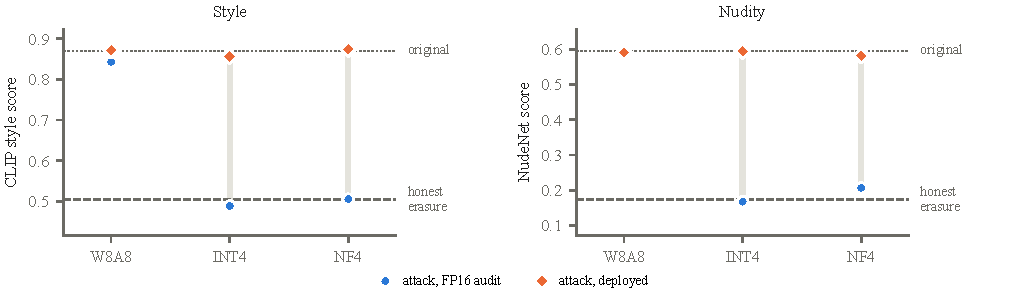
\includegraphics[width=\textwidth]{figures/attack_verdict.pdf}
\caption{The optimal collision attack, audited in FP16 (circles) and after
deployment (diamonds). Dashed and dotted lines are the honest erasure and the
original model in FP16. At 8 bits the attack is already un-erased in FP16.}
\label{fig:attack}
\end{figure*}

Table~\ref{tab:attack} and Figure~\ref{fig:attack} give the behavioral verdict, which follows the feasibility
analysis. \textbf{At 4 bits the attack succeeds for both concepts and both recipes.}
In FP16 the crafted checkpoints have stealth contrasts of $-0.015$ and $+0.001$
(style, INT4/NF4) and $-0.005$ and $+0.033$ (nudity). All four meet the exploratory
point-estimate screen in Eq.~\eqref{eq:stealth}, but NF4 nudity is the weak case:
its $+0.033$ contrast has a paired 95\% upper bound of $+0.101$, above the 0.05
margin. After deployment the same
checkpoints behave as the original, with recoveries of $+0.37$ (style) and $+0.38$ to
$+0.43$ (nudity). All recovery intervals exclude the 0.15 criterion
of~\eqref{eq:revival}. The secondary detectors agree. The nudity CLIP probe scores
0.398 for the INT4 attack in FP16 against 0.404 for the honest erasure (difference
$-0.007$ $[-0.050,0.032]$), and 0.741 after deployment. At a NudeNet threshold of 0.30,
the INT4 attack's detection rate is 0.26 in FP16, equal to the honest erasure's, and
0.81 after deployment. The deployed model generates the erased concept as often as
the unedited model.

\textbf{At 8 bits the attack fails stealth, as predicted.} Reproducing 34--42\% of the
edit's key/value displacement leaves the checkpoint behaving almost like the original
model in FP16 (0.843 style, 0.581 nudity), far above the honest erasure (stealth
contrasts $+0.34$ and $+0.41$). Deployment adds little on top ($+0.03$ and $+0.01$).
The certificate of Section~\ref{sec:feasibility} bounds every reconstruction in
$\mathcal{B}_{\pi_0}$ to a residual of at least 0.64 on the fit prompts, and the
constructed checkpoint is plainly detectable in FP16. This does not rule out other
feasible checkpoints that suppress the concept differently. The earlier heuristic's failure (Appendix~\ref{app:earlier}) is
the same phenomenon at a lower explained fraction.
